\chapter[Introdução]{Introdução}

O malte é um produto de extrema importância para diversos setores industriais, com ele sendo o principal insumo na produção de cerveja, onde fornece açúcares fermentáveis, cor e aroma à bebida. No setor cervejeiro, o malte de cevada é o mais utilizado; no entanto, há um crescente interesse em pesquisas que buscam desenvolver malte a partir de outros grãos, como arroz, milho e trigo, visando atender demandas específicas, como a produção de cervejas livres de glúten \cite{CECCARONI2019}. Além disso, o malte tem ganhado destaque como ingrediente funcional na indústria alimentícia, sendo utilizado, por exemplo, na fabricação de pães, devido às suas propriedades nutricionais \cite{KOISTINEN2020}.

A produção de malte, no entanto, enfrenta desafios significativos, especialmente em climas quentes, onde o controle preciso de temperatura, umidade e tempo, durante as etapas de maceração, germinação e secagem, é crucial para garantir a qualidade do produto \cite{KOVALOVA2024}. O controle desses parâmetros torna a malteação um processo complexo, exigindo equipamentos especializados e sistemas automatizados para otimizar a produção. No contexto acadêmico e de pesquisa, a falta de equipamentos acessíveis e confiáveis para malteação em laboratório limita o desenvolvimento de estudos e inovações nesta área, evidenciando a importância de soluções de baixo custo.
% A base dessa minha afirmação "forte" foram minhas pesquisas mais diretas por equipamentos, que normalmente são industriais. Essa é a forma que encontrei para justificar o trabalho, não sei se foi a melhor abordagem, mas parece funcionar. - Nicolas

Nesse contexto, um dos principais desafios enfrentados é a falta de equipamentos que permitam a malteação controlada em laboratório, comprometendo a precisão e a reprodutibilidade dos experimentos. Durante uma iniciação científica (IC), foi desenvolvido um protótipo inicial (\autoref{fig:malteador}), não finalizado, restando completar a montagem física e desenvolver o sistema de controle e automação. O presente trabalho dá continuidade à IC ao propor uma solução de \textit{software} responsável por garantir que o processo de malteação ocorra adequadamente. 
% A minha intenção é que essa última frase exponha os objetivos do trabalho. - Nicolas

\begin{figure}[ht]
    \centering
    \caption{Protótipo desenvolvido durante a IC. (A) Interface, placa de desenvolvimento e relés das válvulas; (B) Relé de estado sólido; (C) Parafuso de revolvimento; (D) Entrada de ar; (E) Entrada de água; (F) Saída de água; (G) Sensor de dióxido de carbono, umidade e temperatura.}  
    \label{fig:malteador}
    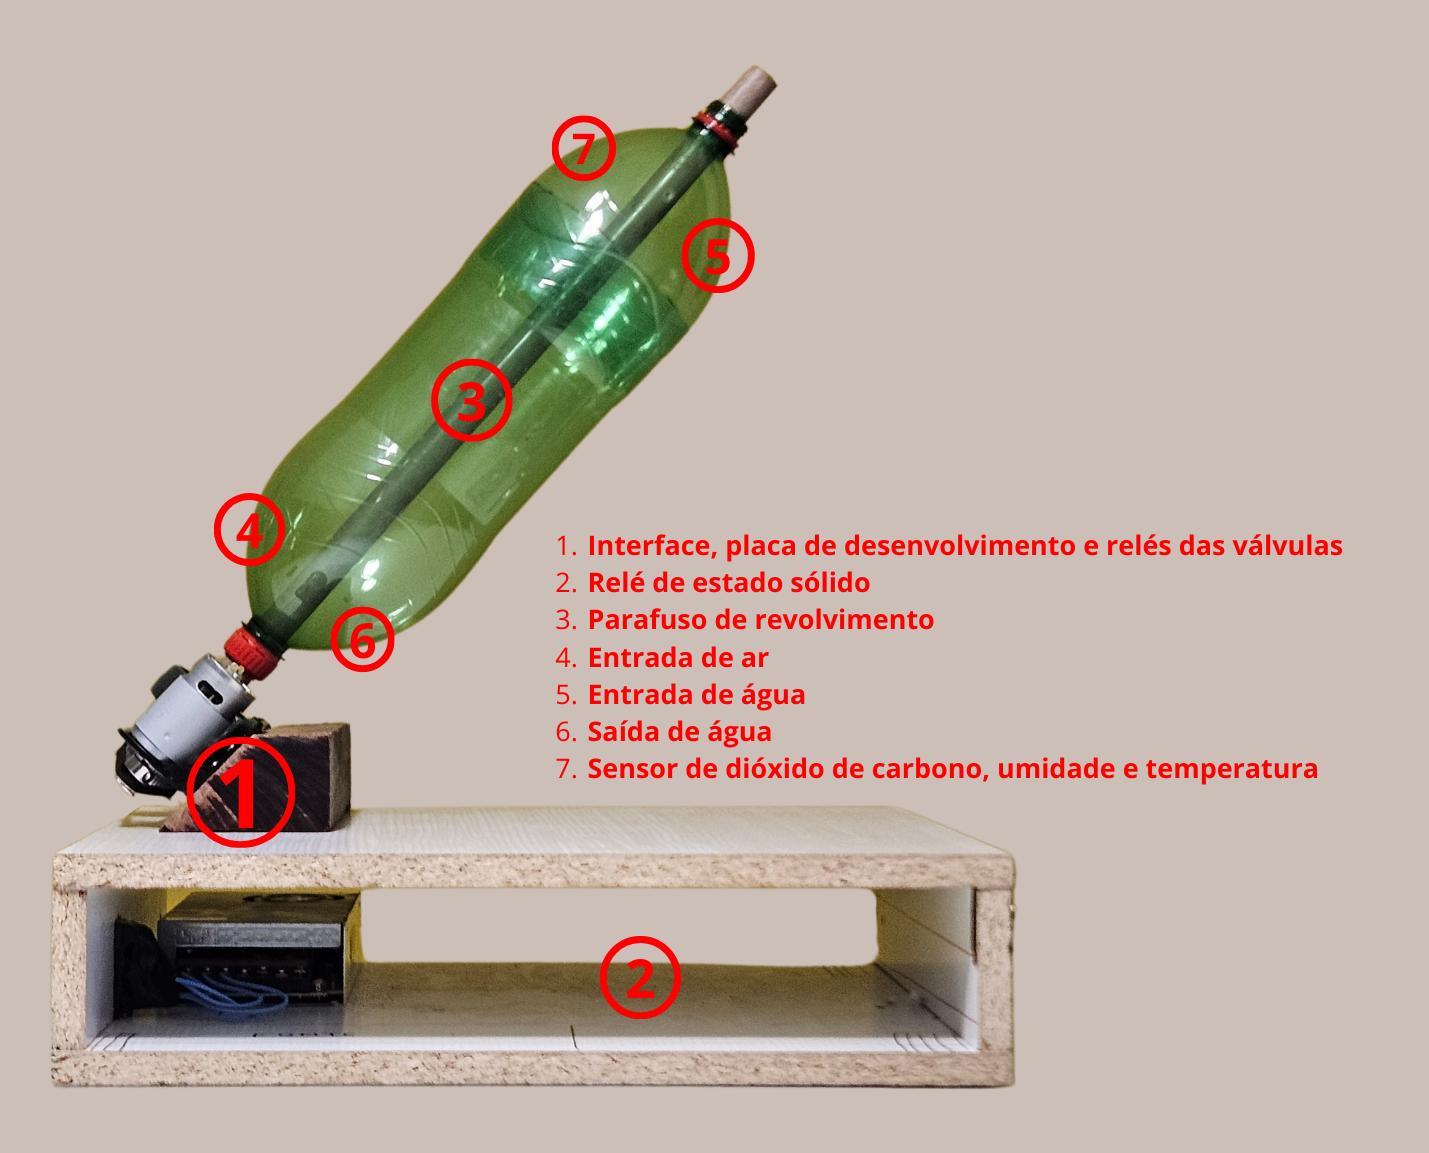
\includegraphics[width=0.8\textwidth]{Vista Lateral do Malteador.png}

    {\centering\footnotesize Fonte: Autoria própria.\par}
\end{figure}

A proposta visa o desenvolvimento de um sistema (\autoref{fig:esquemaeletronico}) baseado no microcontrolador ESP32-C3, da fabricante chinesa Espressif Systems, integrado com um aplicativo Android. Esse microcontrolador foi escolhido por sua relação custo-benefício, capacidade de processamento e suporte a tecnologias de comunicação como Bluetooth e Wi-Fi \cite{rodrigues2021controle, santos2019sistema}. Para seu firmware, optou-se pela linguagem MicroPython, que oferece uma curva de aprendizado suave e é bastante utilizada em projetos de prototipagem rápida e Internet das Coisas (IoT) \cite{TOLLERVEY2017, brito2020automaccao}. Já o aplicativo Android foi desenvolvido em Kotlin, linguagem oficial para o desenvolvimento Android \cite{sempreupdate_kotlin_2020}. A comunicação entre o firmware e o aplicativo é realizada via Bluetooth Low Energy (BLE), uma tecnologia de baixo consumo energético e amplamente disponível em dispositivos móveis \cite{heydon2012bluetooth}, permitindo a configuração remota e o monitoramento em tempo real dos parâmetros operacionais. Além disso, a documentação dos softwares desenvolvidos pode servir como referência para outros estudos envolvendo IoT dentro do IFES, especialmente no que se refere à integração entre ESP32 e Android.
% Adicionei referências a esse parágrafo. - Nicolas

\begin{figure}[ht]
    \centering
    \caption{Esquema eletrônico do malteador desenvolvido durante a IC: (A) relés para atuação das válvulas; (B) relés para atuação do motor e da resistência elétrica; (C) sensor de umidade, temperatura e dióxido de carbono; (D) painel LCD; (E) botão de emergência; (F) microcontrolador ESP32}
    \label{fig:esquemaeletronico}
    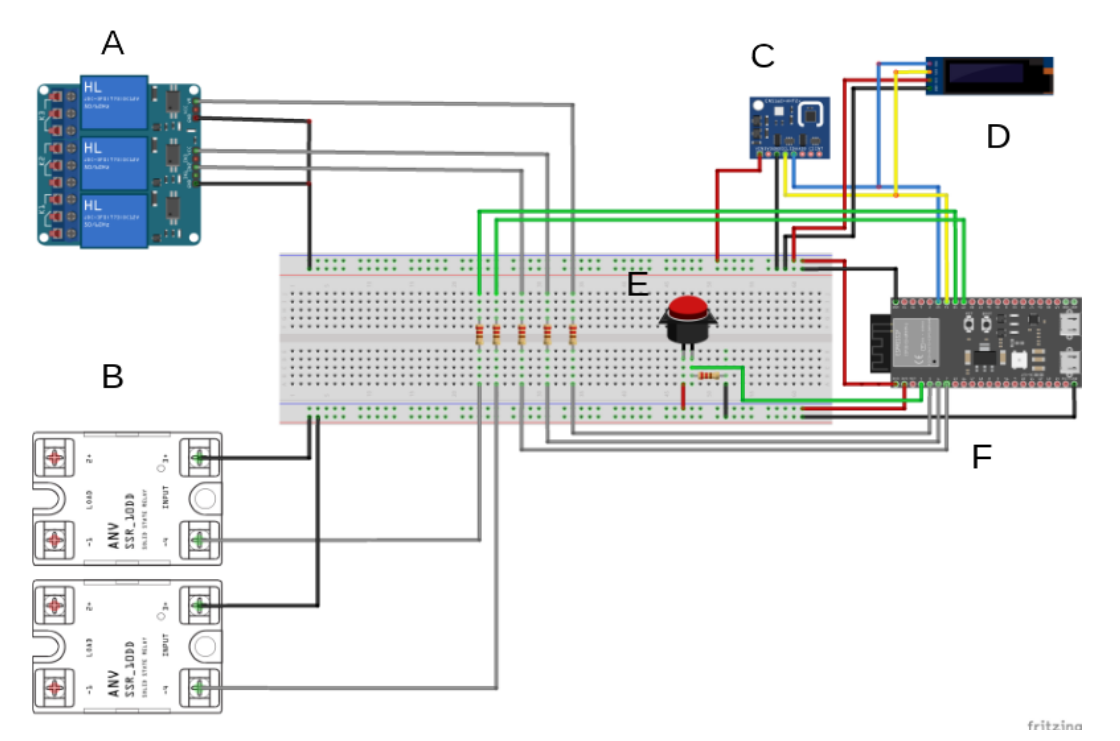
\includegraphics[width=0.8\textwidth]{esquemaeletronico.png}

    {\centering\footnotesize Fonte: Autoria própria.\par}
\end{figure}


Este trabalho surge a partir da demanda do Laboratório de Análises de Cerveja e Matérias-Primas (LACEMP), que busca iniciar estudos experimentais sobre o processo de malteação. A ausência de um equipamento adequado e acessível para pesquisas acadêmicas motivou o desenvolvimento de um sistema que permita monitorar e controlar as variáveis do processo de forma precisa e reprodutível. 

Por fim, a automação proposta busca simplificar a operação do equipamento e fornecer dados estruturados sobre o processo, facilitando futuras análises e ajustes nos experimentos conduzidos no LACEMP. Com isso, espera-se que esta solução de baixo custo promova avanços tanto na pesquisa acadêmica quanto no desenvolvimento de tecnologias acessíveis para a indústria cervejeira e áreas afins.